\chapter{FUNDAMENTAÇÃO TEÓRICO-METODOLÓGICA}

<<<<<<< .mine
Atualmente com o sequenciamento de genomas de varias espécies, muitos estudos estão sendo realizados para descifrar o funcionamento e comportamento das células. Muitos avanços no estudo envolvendo genomas foram alcançados, como por exemplo a caracterização de genes. Mas ainda resta muito trabalho para entender a informação inserida no genoma de um organismo.
=======
>>>>>>> .r3

<<<<<<< .mine
Uma das atividades da célula, que ainda está distante de ser completamente entendida, é a regulação da expressão gênica. O entendimento da regulação dos genes irá trazer benefícios para as pesquisas como a de tratamento e prevenção de doenças. Para entendê-la é essencial a identificação dos elementos regulatórios, uma vez que para que a transcrição de um gene ocorra é necessário a ação destes elementos. O entendimento dos elementos regulatórios é um passo fundamental para a compreensão da regulação de um gene.
=======
O primeiro passo na expressão de um gene é a transcrição. No processo de transcrição muitos fatores internos ou externos, na célula, podem influenciar induzindo ou reprimindo a expressão dos diversos genes codificados no genoma do organismo. Fatores externos desafiantes, como estresses bióticos e abióticos, até mecanismos moleculares intrínsecos podem desencadear, direta ou indiretamente, a ativação da expressão gênica espaço-temporal.

%achar definições em livros para complementar inserir uma figura para explicar visualmente
A transcrição consiste na formação do RNA a partir do DNA, para que a transcrição ocorra é necessário a ação de uma enzima chamada RNA-polimerase, essa enzima se conecta na sequência de DNA, próximo a região onde está o local de inicio da transcrição (LIT) e se move sobre o DNA, no sentido contrario ao LIT formando o RNA, a transcrição é iniciada exatamente após o LIT. Por sua vez para que a RNA-polimerase consiga se conectar no DNA é imprescindível a ação conjunta de proteínas especiais que se conectam a determinados segmentos de DNA.

% pesquisar sobre fatores de transcrição basicos para a transcrição
Essas proteínas são chamadas de fatores de transcrição (TFs), elas podem se conectar distante da RNA-polimerase ou próximo a RNA-polimerase formando um complexo de vários fatores de transcrição juntamente com a RNA-polimerase. Os segmentos de DNA em que os TFs se ligam são pequenos(5 a 20 nucleotídeos), e são chamados de elementos regulatórios. Geralmente os elementos regulatórios estão  localizados em uma região antes do local de inicio da transcrição, como mostrado na figura 1. Esta região recebe o nome de região promotora, ela será responsável de promover um gene, para ser expresso. A ligação dos TFs nos elementos regulatórios interfere no posicionamento correto da RNA-polimerase, na separação das fitas de DNA para permitir o inicio da transcrição, e na liberação da RNA-polimerase quando a transcrição se inicia e consequentemente na transcrição de um gene. Quando ocorre a transcrição parte do RNA transcrito ira formar posteriormente proteínas, que são essenciais para a sobrevivência do organismo, estas proteínas podem até mesmo ser TFs que irão ativar outros genes.

A transcrição esta diretamente ligada a respostas das células a estímulos, como mudanças hormonais internamente em um organismo, ou externamente como estresses abióticos e bióticos. Os estresses abióticos são causados por fatores não vivos como a alteração de temperatura e mudança climática. Os estresses bióticos são causados por organismos vivos como bactérias, vírus, parasitas e insetos.


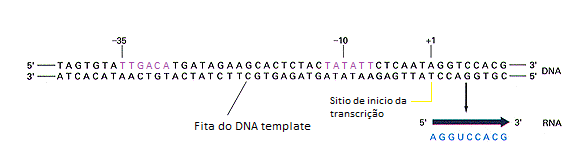
\includegraphics[]{imagens/regiaopromotora}
>>>>>>> .r3

<<<<<<< .mine
Para a identificação dos elementos regulatórios, foram propostos vários métodos, mas ainda não existe um método livre de falhas. Nas seções seguintes serão explicados o início da regulação de um gene e o papel dos elementos regulatórios na regulação de um gene. Também serão apresentados as metodologias computacionais que são adotadas atualmente para a identificação dos elementos regulatórios.

\section{Início da regulação de um gene}

O primeiro passo na expressão de um gene é a transcrição. No processo de transcrição muitos fatores internos ou externos, na célula, podem influenciar induzindo ou reprimindo a expressão dos diversos genes codificados no genoma do organismo. Fatores externos desafiantes, como estresses bióticos e abióticos, até mecanismos moleculares intrínsecos podem desencadear, direta ou indiretamente, a ativação da expressão gênica espaço-temporal.

\subsection{Ácidos nucleicos}
Os ácidos nucleicos são moléculas que exercem um importante papel nos organismos vivos. Neles estão contidos as informações genéticas da célula. É a partir deles que as células recebem instruções de quais proteínas sintetizar e em que quantidade. Essa informação é decifrada através do código genético, cuja a tradução resulta na síntese de proteínas \cite{Zaha2000}.
Existem dois tipos de ácidos nucleicos: ácido desoxirribonucleico (DNA) e ácido ribonucleico (RNA), ambos os ácidos são compostos por nucleotídeos. Os nucleotídeos são formados a partir de três componentes químicos: um açúcar, uma base nitrogenada e um ácido fosfórico (figura \ref{fig:nucleotideo}). Os nucleotídeos estão ligados entre eles formando uma sequência linear (figura \ref{fig:sequencia_nucleotideo}).

\begin{figure}[htb!]
    \centering
    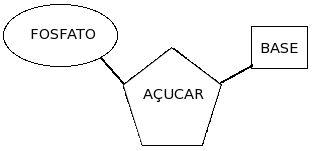
\includegraphics[scale=0.7]{./imagens/componentes_nucleotideo.png}
    \caption{Componentes de um nucleotídeo}
    \label{fig:nucleotideo}
\end{figure}

\begin{figure}[htb!]
    \centering
    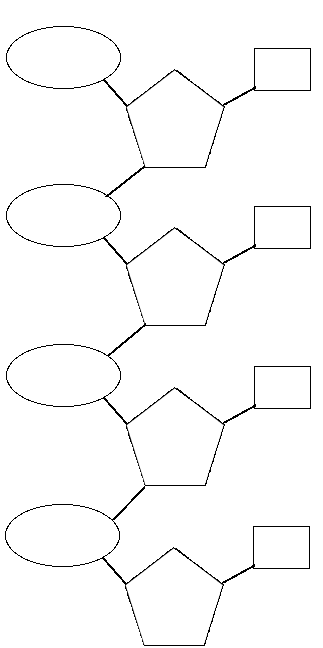
\includegraphics[scale=0.5]{./imagens/sequencia_nucleotideo.png}
    \caption{Sequência linear de nucleotídeos ligados}
    \label{fig:sequencia_nucleotideo}
\end{figure}

Existem duas importantes diferenças entre o RNA e o DNA, que são: o tipo de açúcar e as bases nitrogenadas. O açúcar no DNA é a desoxirribose e no RNA a ribose (figura \ref{fig:tipos_acucar}). Em cada ácido nucleico são encontradas quatros bases nitrogenadas, sendo que três delas são compartilhadas entre o RNA e DNA são elas: adenina (A), guanina (G) e citosina (C). A base timina (T), é encontrada só no DNA, e a uracila (U), é encontrada só no RNA. Porém existe outra grande diferença entre o RNA e o DNA no nível estrutural. O RNA geralmente existe como uma única sequência de nucleotídeos, enquanto o DNA existe como duas sequências de nucleotídeos pareadas que formam um helicoide, conhecido como dupla hélice. Na figura \ref{fig:estrutura_DNA_RNA}, podemos observar a estruturas dos dois ácidos. As bases nitrogenadas no DNA estão no interior da hélice, ligadas por pontes de hidrogênio formando pares de bases nitrogenadas (pb). Os únicos pares possíveis no DNA são: A ligado com T e C ligado com G \cite{Zaha2000}.

\begin{figure}[htb!]
    \centering
    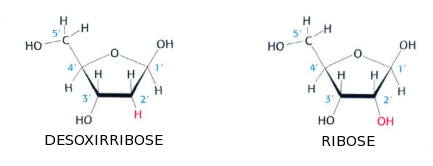
\includegraphics[scale=0.7]{./imagens/tipos_acucar.png}
    \caption{Tipos de açúcar encontrados nos ácidos nucleicos. \cite[Adaptada]{Berg2007})}
    \label{fig:tipos_acucar}
\end{figure}


\begin{figure}[htb!]
    \centering
    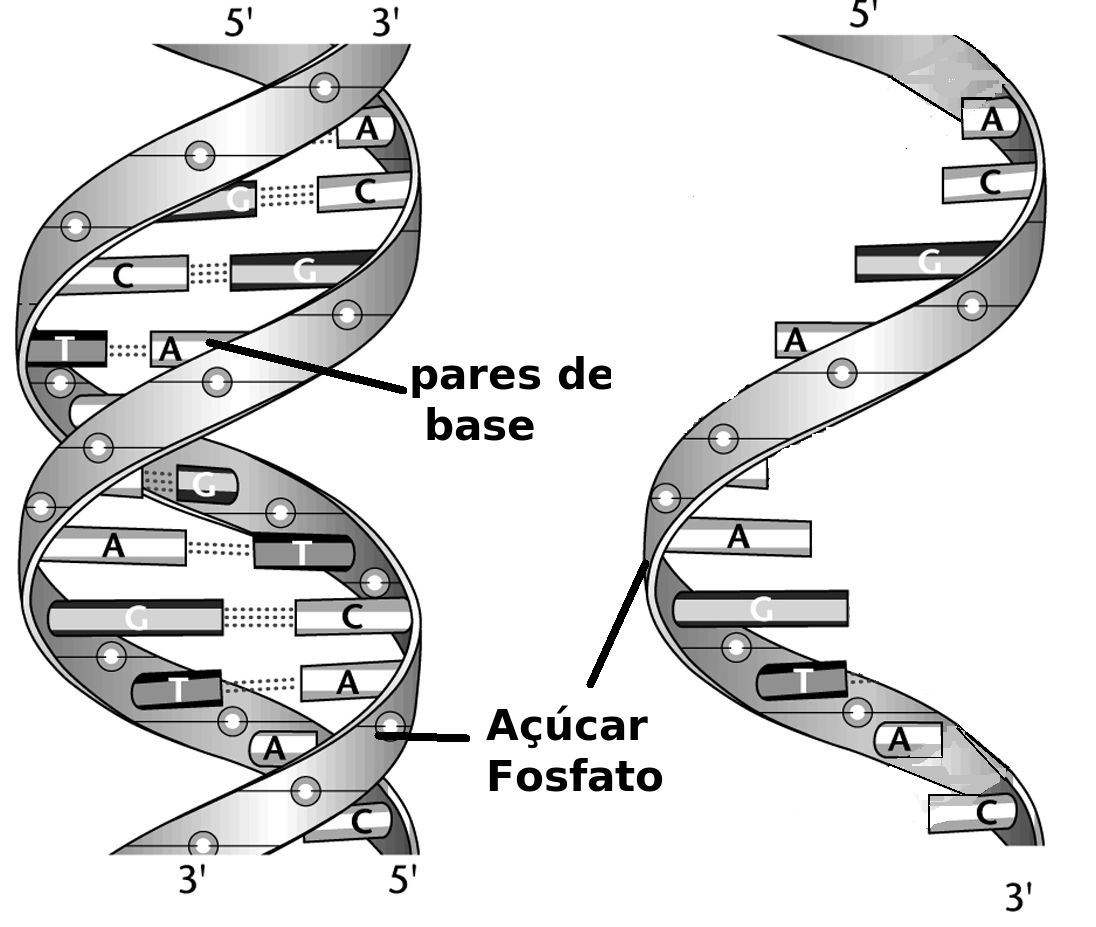
\includegraphics[scale=0.7]{./imagens/estrutura_DNA_RNA.jpg}
    \caption{Estrutura do DNA e RNA. \cite[Adaptada]{Higgs2005}}
    \label{fig:estrutura_DNA_RNA}
\end{figure}



O RNA apesar de ter apenas uma cadeia de nucleotídeos também tem bases complementares. Na síntese de RNA, descrita com mais detalhes na seção 2.1.2, as bases que compõem a sequência do RNA são o complemento das bases copiadas do filamento (sequência de nucleotídeos) do DNA modelo, com a substituição de T por U no RNA . As bases complementares no RNA são: A ligado com U e C ligado com G.


A figura \ref{fig:repre_sequencia}, mostra uma sequência de DNA e uma de RNA. Elas são comumente representas como uma palavra formada pelo alfabeto (A, G, C, T), para representações de DNA e (A, G, C, U), para representações do RNA. A leitura é feita da esquerda para a direita, no sentido indicado como 5'-> 3'. Este tipo de representação torna fácil a visualização, assim como a manipulação a nível computacional, sendo amplamente utilizado em métodos \textit{in silico} que envolvem o DNA e o RNA.

\begin{figure}[htb!]
    \centering
    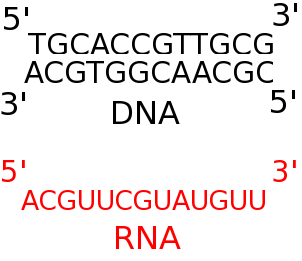
\includegraphics[scale=0.7]{./imagens/repre_sequencia.png}
    \caption{Reapresentação do RNA e DNA}
    \label{fig:repre_sequencia}
\end{figure}

A interação entre o RNA e DNA ocorre quando é necessário a expressão de um gene. A expressão genética inicia-se por um processo chamado transcrição detalhado na seção 2.1.2. Neste processo ocorre a formação do RNA (síntese de RNA), a partir de um dos filamentos do DNA. A sequência de RNA formada é uma cópia exata de uma região do RNA. Esta região que é copiada é chamada de gene. Os genes são seguimentos de DNA podendo ter milhares de pares de bases. São eles que irão especificar o tipo de proteína a ser sintetizado. O processo da síntese de proteínas é conhecido como tradução. A figura \ref{fig:passo_expresscao_genica}, apresenta cada passo deste conjunto de processos, que também é comumente conhecido como o dogma central.
% talvez falar sobre a importancia da expressão genica

\begin{figure}[htb!]
    \centering
    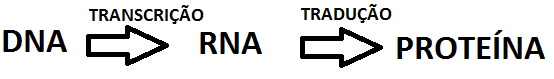
\includegraphics[scale=0.7]{./imagens/passo_expresscao_genica.png}
    \caption{Principais passos da expressão de genética}
    \label{fig:passo_expresscao_genica}
\end{figure}


\subsection{ Transcrição e a síntese de RNA}


Todo o RNA é formado a partir do DNA em um processo chamado transcrição. A transcrição começa com a abertura da hélice dupla do DNA e um dos filamentos do DNA servirá como modelo para a síntese de RNA. A sequência de nucleotídeos na cadeia de RNA é determinada pelo complemento do molde do filamento de DNA (figura \ref{fig:seq_DNA_molde_e_nao_model}). Para que ocorra a formação do RNA é necessário a ação de uma enzima que realiza a transcrição, ela é chamada de RNA polimerase. A RNA polimerase se conecta no DNA, então ela move-se ao longo do DNA na direção 5' para a 3', formando a cadeia de RNA que vai se alongando de um nucleotídeo por vez, terminando com uma sequência de nucleotídeos exatamente complementar ao filamento de DNA usado como modelo (figura \ref{fig:RNAPOLII}).  Após terminada a cópia a cadeia de RNA, juntamente com a RNA polimerase, se desconectam e ocorre o fechamento da hélice do DNA. O RNA formado possuí apenas um filamento e é menor do que uma molécula de DNA. Uma molécula de DNA no cromossomo humana pode ser maior que 250 milhões de pares de nucleotídeos, a maioria das moléculas de RNA não passam de poucos milhares de nucleotídeos.

\begin{figure}[htb!]
    \centering
    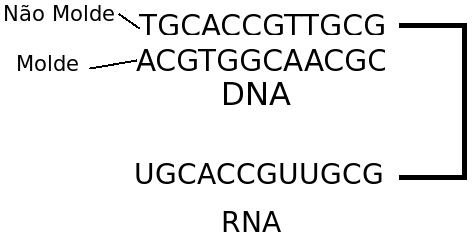
\includegraphics[scale=0.7]{./imagens/seq_DNA_molde_e_nao_model.png}
    \caption{RNA formado, complementar ao filamento modelo}
    \label{fig:seq_DNA_molde_e_nao_model}
\end{figure}


Nos organismos eucarióticos existem três RNA polimerase, chamadas de RNA polimerase I, RNA polimerase II, RNA polimerase III. As três enzimas são similares umas com as outras. A maior diferença entre elas é o tipo de gene que elas transcrevem. RNA polimerase I e III transcrevem os genes que codificam o RNA transportador (transporta aminoácidos que se interagem com o RNA mensageiro formando as proteínas)  e RNA ribossômico (um conjunto de RNA ribossômico forma o ribossomo, uma estrutura necessária na síntese da proteína), respectivamente. A RNA polimerase II transcreve a maioria dos genes, ela gera o RNA mensageiro, utilizado na formação das proteínas. Para que a RNA polimerase inicie a transcrição é necessário um grande conjunto de proteínas chamadas de fatores de transcrição gerais.

\begin{figure}[htb!]
    \centering
    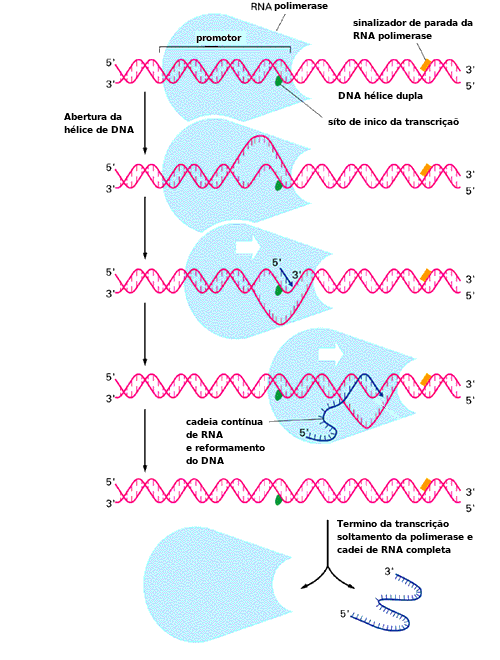
\includegraphics[scale=0.7]{./imagens/RNAPOLII.png}
    \caption{Formação do RNA através da RNA polimerase \cite[Adaptada]{Higgs2005}}
    \label{fig:RNAPOLII}
\end{figure}



Os fatores de transcrição gerais se conectam em pontos de ligação na sequência de DNA chamados de promotores. Os promotores são pequenos segmentos de DNA, reconhecidos pela RNA polimerase, que servem como sinalizadores para o posicionamento correto da RNA polimerase. Eles estão localizados pouco antes do gene que será transcrito pela RNA polimerase. É nos promotores que a RNA polimerase se conecta, juntamente com os fatores de transcrição gerais para iniciar a transcrição. Logo após os promotores, está o local de inicio da transcrição (TSS, do inglês \textit{transcription start site}), este é o local onde inicia-se a transcrição, ou seja o primeiro nucleotídeo a ser transcrito e a sua posição é marcada como +1, todos os nucleotídeos antes são marcados com suas posições com números iniciando-se pelo -1 negativos (-1, -2, -3...), e após com números positivos. Na figura \ref{fig:complexo_RNA-polimerase}, podemos visualizar os promotores antes do TSS, assim como a RNA polimerase e os fatores de transcrição gerais se conectando na sequência de DNA.

\begin{figure}[htb!]
    \centering
    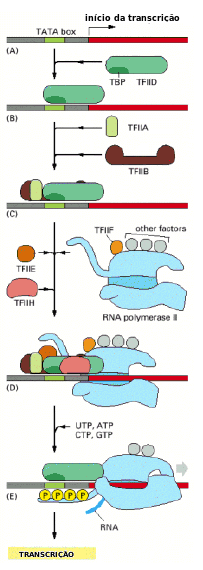
\includegraphics[scale=0.7]{./imagens/complexo_RNA-polimerase.png}
    \caption{RNA polimerase e os fatores de transcrição gerais \cite[Adaptada]{Alberts2002} }
    \label{fig:complexo_RNA-polimerase}
\end{figure}

Os promotores seguem um padrão, e geralmente ele é o mesmo para os promotores da maioria dos genes. Por exemplo em muitas bactérias, na região promotora (região do DNA onde encontra-se os promotores de um gene) da maioria dos genes, existe uma sequência que tem como consenso a sequência \textbf{TATAATT} localizada aproximadamente na região -10. Outra sequência é a \textbf{TTGACA} localizada aproximadamente na região -35 (figura \ref{fig:promotores_noDNA}).

\begin{figure}[htb!]
    \centering
    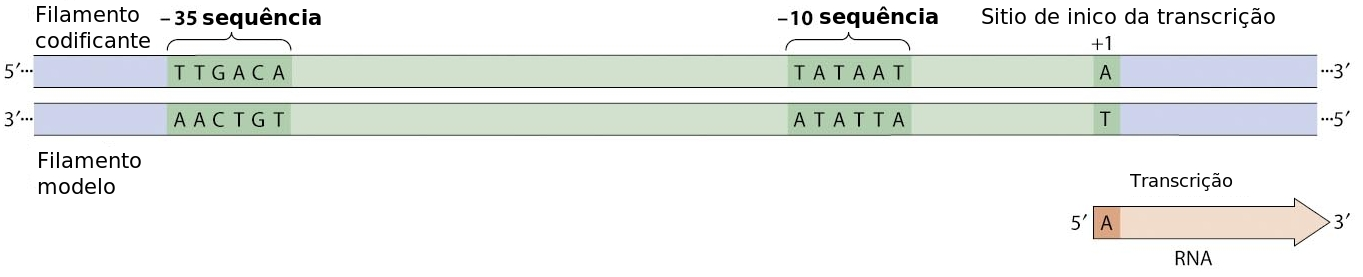
\includegraphics[scale=0.7]{./imagens/promotores_noDNA.jpg}
    \caption{Região promotora e as sequências consenso}
    \label{fig:promotores_noDNA}
\end{figure}


A ligação dos fatores de transcrição gerais nos promotores, ajuda no correto posicionamento da RNA polimerase, na separação dos dois filamentos de DNA para permitir o inicio da transcrição, e lançar a RNA polimerase do promotor para iniciar a transcrição. Os fatores de transcrição são ditos gerais porque, eles se ligam a todas as regiões promotoras usada pela RNA polimerase II. Estes fatores de transcrição classificados como TFII (para fatores de transcrição da polimerase II), e listados com TFIIA, TFIIB etc. %inserir uma figura%

O desligamento da RNA polimerase do DNA, no fim da transcrição, não é aleatório. A RNA polimerase encontra novamente sequências consenso conhecidas como finalizadores, então ela se desconecta do DNA, que se fechará, voltando a estrutura original da dupla hélice. O RNA transcrito está pronto ou como o tRNA e rRNA ou como mensagem (mRNA) para ser traduzida em proteínas por meio da tradução.

\subsection{Elementos regulatórios}

Além dos promotores, existem outras sequências no DNA em que fatores de transcrição se conectam. Essas sequências são chamadas de elementos regulatórios(ou promotores proximais), eles ficam aproximadamente uma distância de -50 pares de base do local de início da transcrição \cite{Zaha2000}. Eles se encontram assim como os promotores na região promotora de um gene e também são pequenos (5 a 20 nucleotídeos). Mas diferentes dos promotores os fatores de transcrição(TFs) que conectam a eles não são fatores de transcrição gerais, mas sim específicos. Portanto um fator de transcrição específico utilizado na expressão de um determinado gene, pode não ser o mesmo para a expressão de outro gene. Por exemplo o conjunto de fatores de transcrição de uma célula óssea no organismo humano, pode ter fatores diferentes do conjunto de TFs de uma célula do figado, uma vez que essas diferentes células podem precisar de diferentes proteínas. Essa especificidade torna os elementos regulatórios em sequências que não são consenso, em consequência os elementos regulatórios não seguem um padrão.

Existem elementos regulatórios que são ativados em resposta a estímulos como mudanças hormonais internamente em um organismo, ou externamente como: estresses abióticos que são causados por fatores não vivos como a alteração de temperatura e mudança climática, ou estresses bióticos causados por organismos vivos como bactérias, vírus, parasitas e insetos. Com a ativação do elemento regulatório ocorrera a expressão do gene, que o elemento regula, o gene será transcrito no RNA que posteriormente será traduzido, gerando proteínas para suprir as necessidades do organismo.

\subsection{Fatores de transcrição que ativam elementos regulatórios em resposta a estresses abióticos}

No amplo conjunto de fatores de transcrição, existem aqueles que quando ligados nos elementos regulatórios irão ativar as respostas da célula a estresses abióticos. O estresse abiótico afeta diversos organismos, mas em especial os organismos vegetais que são dependentes de fatores ambientais, são os mais afetados. Em organismos vegetais os estresses abióticos que mais prejudicam são: a seca, alta salinização e baixas temperaturas.

A ligação entre os fatores de transcrição que estão relacionados a expressão de um gene (ou conjunto de genes), com elementos regulatórios, no momento em que o organismo é exposto a um estresse, a célula produzira proteínas, que irão agir na proteção da célula.

Na Arabdopsis, uma planta modelo amplamente utilizada em pesquisas de genética molecular nas plantas. Com estudos em laboratório foram encontrados alguns fatores de transcrição relacionados a estresses abióticos, eles são agrupados em classes (ou famílias). Atualmente uma das classes que vem sendo objeto de muitos estudos, devido a sua resposta a diversos estresses, é a Dehydration Responsive Element Binding Proteins (DREB) que por sua vez pertence a família Ethylene Responsive Element (ERF), uma importante família de fatores de transcrição de respostas a estresses. Os DREBs desempenham um importante papel na proteção de algumas plantas, provendo tolerância a estresses e respondendo a diferentes condições de estresses, como: frio, alta salinidade e seca \cite{Agarwal2006}.

Segundo Agarwal et al.\cite{Agarwal2006} estresses abióticos e bióticos influenciam negativamente na sobrevivência e na larga produção de grãos. Culturas como soja, arroz e trigo que são amplamente usadas na alimentação mundial são prejudicadas pelos estresses que muitas vezes impedem uma alta produtividade. O entendimento dos DREBs na regulação de um gene é de grande importância para o desenvolvimento de plantas tolerantes a estresses.

\section{Métodos computacionais para a predição de elementos regulatórios}

Atualmente vários métodos computacionais foram desenvolvidos para detectar elementos regulatórios. Apesar dos avanços para encontrar elementos relatórios, a busca \textit{in silico} não é tão precisa, diferente por exemplo da classificação de genes, gerando muitos resultados falsos. Isto deixa em aberto um vasto campo para ser explorado \cite{Rombauts2003}. Um dos principais problemas na predição de elementos regulatórios, é que eles são definidos funcionalmente e não estruturalmente, limitando os meios para modelá-los \cite{Rombauts2003}. A identificação experimental de elementos regulatórios é  cara, demorada e difícil. Isso faz dos métodos computacionais as ferramentas ideais para predizer elementos regulatórios, antecipando os estudos experimentais de regulação da expressão gênica.


Dos métodos de predição existentes, Das e Dai \cite{Das2007} os classificaram em três grupos:
\begin{itemize}
\item Os baseados em sequências promotoras de genes que são regulados pelos mesmos fatores de transcrição (genes co-regulados); estes métodos se concentram em apenas um único genoma.

\item Os que utilizam sequências promotoras de genes ortólogos, que são sequências de DNA similares a várias espécies, indicando que estas espécies derivaram de um ancestral comum, também chamados de métodos de rastros filogenéticos.

\item Os métodos que combinam rastros filogenéticos e sequências promotoras de genes co-regulados.
\end{itemize}


Os métodos baseados em genes co-regulados ainda podem ser divididos em dois subgrupos: de predição baseada em palavras e predição probabilística.


\subsection{Algoritmos de predição baseada em palavras}

Os algoritmos de predição baseada em palavras, geralmente utilizam de enumeração exaustiva, computando todas as possíveis subsequências que podem ocorrer, através de diferentes sequências promotoras, ou de árvores sufixa, que representam as sequências promotoras em uma árvore sufixa. Ambas as abordagens tem o objetivo de encontrar número de frequência de uma subsequência, o qual deve ser comparado com o número de frequência esperada. Nesta etapa, são utilizados métodos estatísticos para avaliar a significância da sequência observada \cite{Rombauts2003}.

Uma das primeiras abordagens de predição baseada em palavras é a Oligo-Analysis um algoritmo desenvolvido por Helden \textit{et al}. \cite{Helden1998}. O algoritmo desenvolvido foi utilizado na predição de elementos regulatórios em leveduras( \textit{Saccharomyces cerevisiae}), as sequências promotoras utilizadas foram de genes co-regulados, e para o cálculo da frequência foi usado o método de enumeração exaustiva. O algoritmo mostrou-se eficiente na busca de elementos regulatórios pequenos e altamente conservados.



\subsection{Algoritmos de predição probabilística}

Os modelos de predição probabilística, geralmente utilizam matriz de peso e os parâmetros do modelo são estimados usando o princípio de inferência bayesiana. Há varias implementações baseadas no método probabilístico, entre estas técnicas destacam-se as técnicas estatísticas como \textit{EM (Expectation-maximization algorithm)} método e \textit{Gibb sampling}, técnicas de aprendizado de máquina e técnicas de \textit{Ensemble} \cite{Das2007}.

A introdução do EM para a busca de elementos regulatórios foi feita por Lawrence e Reilly \cite{Lawrence1990}. O algoritmo assume que cada sequência tem pelo menos um elemento em comum. Diferente de outros algoritmos, neste algoritmo não é necessário o alinhamento das sequências.

Nos modelos de predição probabilística que utilizam técnicas de aprendizado de maquina, uma das técnicas que vem mostrando grande eficiência na busca de elementos regulatórios é a de \textit{support vector machine} (SVM). Wang \textit{et al.} \cite{Wang2009} utilizaram sequências de DNA de regiões promotoras da \textit{Arabidopsis}, que continham elementos regulatórios que se conectavam a TFs, de genes que eram ativados quando a planta é exposta ao estresse abiótico, e sequências aleatórias da região promotora. Foi aplicado então o algoritmo HexDiff \cite{Chan2005}, este algoritmo encontra novos elementos regulatórios a partir de elementos já conhecidos, com elementos regulatórios encontrados ele então classificou-os com o SVM quais eram ativados em resposta ao estresse abiótico.

Hu \textit{et al.} \cite{Hu2005}, propôs um algoritmo um algoritmo ensemble, que combina múltiplos algoritmos de identificação de elementos regulatórios. Os algoritmos usados foram AlingACE \cite{Roth1998} , Bioprospector \cite{LiuBrutlag2001}, MDScan\cite{LiuBrutlag2002}, MEME \cite{Bailey2006} e MotifSampler \cite{Thijs2002}. Este algoritmo segundo os autores,tem um grande desempenho, mas os resultados são mais precisos na identificação de elementos regulaórios pequenos.

\subsection{Algoritmos baseados em rastros filogenéticos}

Os algoritmos baseados em rastros filogenéticos assumem que elementos regulatórios são regiões conservadas no DNA e não sofreram muitas mutações ao longo da evolução. Esses algoritmos comparam sequências promotoras de genes ortólogos de múltiplas espécies para identificar os elementos regulatórios.

Blanchette \textit{et al.} \cite{Blanchette2002}, desenvolveram o FootPrinter. Este algoritmo que tem como entrada as sequências promotoras de várias espécies e a árvore filogenética das espécies relacionadas. As sequências de cada espécie são inseridas nas folhas da árvore, então são feitas varias comparações das sequências, a começar das folhas. As sequências de tamanho \textit{k}, mais conservadas são promovidas para o nível acima da árvore, são feitas novas comparações até ser atingido a raiz da árvore, chegando a sequências ótimas, que passarão por mais comparações, desta vez da raiz até as folhas, finalizando o algoritmo com os elementos preditos.

\subsection{Algoritmos que combinam técnicas probabilísticas e de rastros filogenéticos}

Por último os algoritmos que combinam as técnicas probabilísticas e de rastros filogenéticos, que integram dois importantes aspectos dos elementos regulatórios, a sobre-representação e a conservação dos elementos regulatórios entre múltiplas espécies \cite{Das2007}.

Sinha \textit{et al.} \cite{Sinha2004}, propuseram um algoritmo combinando as técnicas probabilísticas e de rastros filogenéticos. O algoritmo permite a entrada de sequências promotoras de genes ortólogos, relacionadas com a árvore filogenética definida pelo usuário. As sequências dos elementos regulatórios podem ser conservadas ou não conservadas, o algoritmo as trata de maneira diferente. O algoritmo permite uma flexibilidade, na escolha da árvore filogenética, podendo escolher espécies distantemente relacionadas, que além da identificação dos elementos conservados entre as espécies possibilita a identificação de elementos que não estão relacionados com as especies ortólogas.


Na tabela \ref{tab:metodos_busca_elementos}, estas listados alguns dos algoritmos dos modelos citados.

\begin{table}[h!]
\begin{center}
  \begin{tabular}{| l | c | }
    \hline
    Algoritmos     & Referências       \\ \hline \hline

    \multicolumn{2}{|c|}{Algoritmos de predição baseada em palavras}  \\ \hline

    Oligo-Analysis & \cite{Helden1998} \\ \hline
    YMF            & \cite{Sinha2003}  \\ \hline
    MITRA          & \cite{Eskin2002}  \\ \hline

    \multicolumn{2}{|c|}{Algoritmos de predição probabilística}       \\ \hline

    MEME           & \cite{Bailey2006}   \\ \hline
    Gibbs sampling & \cite{Lawrence1993} \\ \hline
    AlignACE       & \cite{Roth1998}     \\ \hline
    Motif Sampler  & \cite{Thijs2002}    \\ \hline

    \multicolumn{2}{|c|}{Algoritmos baseados em rastros filogenéticos} \\ \hline

    Footprinter    & \cite{Blanchette2002} \\ \hline
    PHYLONET       & \cite{Wang2005}       \\ \hline
    PhyloScan      & \cite{Carmack2007}    \\ \hline

    \multicolumn{2}{|c|}{Algoritmos baseados em rastros filogenéticos e predição probabilística}             \\ \hline

    OrthoMEME      & \cite{Carmack2007}  \\ \hline
    PhyloCon       & \cite{Wang2003}     \\ \hline
    PhyME          & \cite{Sinha2004}    \\ \hline

    \hline

  \end{tabular}
\end{center}
  \caption{Implementações de modelos de predição}
   \label{tab:metodos_busca_elementos}
\end{table}
=======
Figura 1. Região promotora, com dois elementos regulatórios.


No amplo conjunto de fatores de transcrição, existem aqueles que quando ligados nos elementos regulatórios irão ativar as respostas da célula a estresses abióticos. Em organismos vegetais os estresses abióticos que mais prejudicam são: a seca, alta salinização e baixas temperaturas. Esses fatores de transcrição quando ligados aos elementos regulatórios irão desencadear uma série de eventos que resultara na proteção da célula e sua tolerância a estresses. Na \textit{Arabdopsis}, uma planta modelo amplamente utilizada em pesquisas de genética molecular nas plantas, os fatores de transcrição relacionados a estresses abióticos são agrupados em classes (ou famílias), uma das principais classes é a Dehydration Responsive Element Binding Proteins (DREB), que por sua vez pertence a família Ethylene Responsive Element (ERF), uma importante família de fatores de transcrição de respostas a estresses. O DREB é subdividido em duas subclasses: DREB1/CBF e DREB2 que são induzidas pelo frio e desidratação, respectivamente \cite{Agarwal2006}.

Segundo Agarwal et al.\cite{Agarwal2006} estresses abióticos e bióticos influenciam negativamente na sobrevivência e na larga produção de grãos. Culturas como soja, arroz e trigo que são amplamente usadas na alimentação mundial são prejudicadas pelos estresses que muitas vezes impedem uma alta produtividade. O entendimento dos DREBs na regulação de um gene é de grande importância para o desenvolvimento de plantas tolerantes a estresses.


Existem vários métodos computacionais desenvolvidos para encontrar elementos regulatórios nos genes de diversos organismos, Das e Dai \cite{Das2007} classificou os métodos existentes em três grupos:
\begin{itemize}
\item Os baseados em sequências promotoras de genes que são regulados pelos mesmos fatores de transcrição (genes co-regulados), estes métodos se concentram em apenas um único genoma.

\item Os que utilizam sequencias promotoras ortólogas, que são sequencias de DNA similares a várias espécies, indicando que estas espécies derivaram de um ancestral comum, também chamados de métodos de rastros filogenéticos.

\item Os métodos que combinam rastros filogenéticos e sequencias promotoras de genes co-regulados.
\end{itemize}


Os métodos baseados em genes co-regulados ainda podem ser divididos em dois subgrupos: de predição baseada em palavras e predição probabilística.

%%%%
%Fazer uma tabela listando os principais algoritmos dos três grupos
%%%%
Algoritmos de predição baseada em palavras computam todas as possíveis subsequências que podem ocorrer, através de diferentes sequências promotoras. Encontrado o número de frequência de uma subsequência, este deve ser comparado com o número de frequência esperada. Depois, são utilizados métodos estatísticos para avaliar a significância da sequência observada \cite{Rombauts2003}.

Os modelos de predição probabilística, geralmente utilizam matriz de peso e os parâmetros do modelo são estimado usando o princípio de inferência bayesiana. Há varias implementações baseadas no método probabilístico, entre estas técnicas destacam as técnicas estatísticas como \textit{EM} método e \textit{Gibb sampling}, técnicas de aprendizado de máquina e técnicas de \textit{Ensemble} \cite{Das2007}.

Os algoritmos baseados em rastros filogenéticos assumem que elementos regulatórios são regiões conservadas no DNA e não sofreram muitas mutações ao longo da evolução. Esses algoritmos comparam sequências promotoras de genes ortólogos de múltiplas espécies para identificar os elementos regulatórios.

Por último os algoritmos que combinam as técnicas probabilísticas e de rastros filogenéticos, que integram dois importantes aspectos dos elementos regulatórios, a sobre-representação e a conservação dos elementos regulatórios entre múltiplas espécies \cite{Das2007}. Algumas das implementações dos modelos citados estão listadas na tabela 2.1.

Dos modelos apresentados, a predição baseada em palavras mostrou-se eficiente na busca de elementos regulatórios em organismos eucarióticos mas problemática em organismos procarióticos, devido ao tamanho dos elementos regulatórios nos eucarióticos serem menores do que nos procarióticos. A predição baseada em rastros filogenéticos, mostrou-se muito eficiente em organismos procarióticos, mas é necessário as sequencias de varias espécies, para fazer as comparações, com o avanço do sequenciamento do genoma das espécies este método ficara cada vez mais expressivo. O modelo de predição probabilística também tem-se mostrado eficiente na busca de elementos regulatórios em grandes genomas, uma das técnicas que se destaca com  grande eficiência na busca de elementos regulatórios dentro dos modelos que utilizam aprendizado de máquina é a de \textit{support vector machine} (SVM).

Até o presente momento poucos foram os trabalhos que se dedicaram exclusivamente na busca DREBs nas plantas. Recentemente Wang et al. \cite{Wang2009} criou um método utilizando SVM para encontrar genes que eram expressos quando expostos a fatores abióticos na \textit{Arabidopsis}. Eles utilizaram sequencias de DNA de regiões promotoras de genes da \textit{Arabidopsis}, que possuía elementos regulatórios que se conectavam a DREBs como dados positivos e sequencias aleatórias da região promotora representando os dados negativos, primeiramente foi aplicado o algoritmo HexDiff \cite{Chan2005} para análise dos hexâmeros sobre-representados nas sequencias e então as sequencias promotoras dos genes foram classificadas com o SVM, discriminando os as sequencias de genes que eram alvos de DREBs das que não eram.


\begin{table}[h!]
\begin{center}
  \begin{tabular}{| l | c | }
    \hline
    Algoritmos     & Referências       \\ \hline \hline

    \multicolumn{2}{|c|}{Algoritmos de predição baseada em palavras}  \\ \hline

    Oligo-Analysis & \cite{Helden1998} \\ \hline
    YMF            & \cite{Sinha2003}  \\ \hline
    MITRA          & \cite{Eskin2002}  \\ \hline

    \multicolumn{2}{|c|}{Algoritmos de predição probabilística}       \\ \hline

    MEME           & \cite{Bailey2006}   \\ \hline
    Gibbs sampling & \cite{Lawrence1993} \\ \hline
    AlignACE       & \cite{Roth1998}     \\ \hline
    Motif Sampler  & \cite{Thijs2002}    \\ \hline

    \multicolumn{2}{|c|}{Algoritmos baseados em rastros filogenéticos} \\ \hline

    Footprinter    & \cite{Blanchette2002} \\ \hline
    PHYLONET       & \cite{Wang2005}       \\ \hline
    PhyloScan      & \cite{Carmack2007}    \\ \hline

    \multicolumn{2}{|c|}{Algoritmos baseados em rastros filogenéticos e predição probabilística}             \\ \hline

    OrthoMEME      & \cite{Carmack2007}  \\ \hline
    PhyloCon       & \cite{Wang2003}     \\ \hline
    PhyME          & \cite{Sinha2004}    \\ \hline

    \hline

  \end{tabular}
\end{center}
  \caption{Implementações de modelos de predição}
\end{table}


Atualmente existem poucas ferramentas dedicadas à descoberta de elementos regulatórios em plantas, a maior parte das soluções são baseadas em fungos, mamíferos e insetos como a Drosophila. Das ferramentas dedicadas a plantas a maior parte é baseada na planta modelo Arabidopsis.>>>>>>> .r3
